\section{Appendix}

\subsection{Definitions}
\begin{definition}{(Scaled inverse $\chi^2$ distribution).}\label{def:scaledInverseChi}
  Let $\nu > 0$ and $\tau^2 > 0$ be parameters representing degrees of freedom and scale, respectively. The family of \emph{scaled inverse $\chi^2$ distributions} is characterized by its probability density function, namely
  \begin{align*}
    p(x) \propto x^{-(1 + \nu / 2)} \EXP{\frac{-\nu \tau^2}{2 x}} \quad \text{for} \, x \in (0, \infty) \,,
  \end{align*}
  where the constant of integration is ignored for clarity.
  We write $X \sim \scaledInvChi{\nu, \tau^2}$ to denote that the random variable $X$ follows a scaled inverse $\chi^2$ distribution with parameters $\nu$ and $\tau^2$.
\end{definition}

\begin{definition}{(Conjugate prior).}\label{def:conjugate_prior}
Let the likelihood $p(y \mid \theta)$ be given and assume that the prior distribution $p(\theta)$ is a member of some family $\mathcal{F}$ of probability distributions.
We say that $p(\theta)$ is a \emph{conjugate prior} if the posterior $p(\theta \mid y)$ is also a member of $\mathcal{F}$.
\end{definition}

\subsection{Figures}

\begin{figure}[H]
\begin{center}
\begin{tikzpicture}%
  [vertex/.style={circle,draw=black,fill=white, minimum size=1cm},
  node distance=2.5cm,
  >=latex,
  on grid]
  \node[vertex] (phi) {$\phi$};
  \node[rectangle, draw=black, minimum size=0.9cm,left=2cm of phi] (zeta) {$\zeta$};
  \node[vertex,below left=1.5cm and 2cm of phi] (theta1) {$\theta_1$};
  \node[vertex,below right=1.5cm and 2cm of phi] (thetaJ) {$\theta_J$};
  \node[below=1.5cm of phi] (dots1) {$\dots$};
  \node[rectangle, draw=black, minimum size=0.9cm, left=2cm of theta1] (u1) {$u_1$};
  \node[rectangle, draw=black, minimum size=0.9cm, right=2cm of thetaJ] (uJ) {$u_J$};
  \node[vertex,below=2cm of theta1] (y1) {$y(1)$};
  \node[vertex,below=2cm of thetaJ] (yJ) {$y(J)$};
  \node[rectangle, draw=black, minimum size=0.9cm, left=2cm of y1] (x1) {$x(1)$};
  \node[rectangle, draw=black, minimum size=0.9cm, right=2cm of yJ] (xJ) {$x(J)$};
  \node[below=3.5cm of phi] (dots1) {$\dots$};
  \draw[->]
    (zeta) edge (phi)
    (phi) edge (theta1)
    (phi) edge (thetaJ)
    (u1) edge (theta1)
    (uJ) edge (thetaJ)
    (theta1) edge (y1)
    (thetaJ) edge (yJ)
    (x1) edge (y1)
    (xJ) edge (yJ);
\end{tikzpicture}
\end{center}
\caption{A generic two-level Bayesian hierarchical model depicted as a directed acyclical graph modeling generic observations $y(j)$ in groups $j = 1,\mydots, J$. Circled parameters denote random quantities while parameters contained in squares denote fixed quantities.}
\label{fig:group_sem}
\end{figure}


\begin{figure}[H]
	\centering
	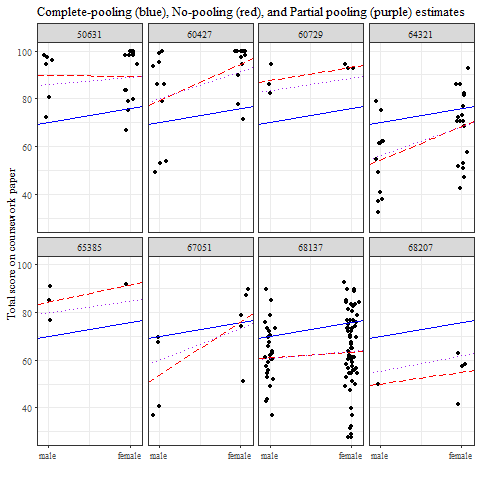
\includegraphics[width=10cm,height=10cm,keepaspectratio]{graphics/pooling.png}
	\caption{We see that the estimated school-specific regression line from the partial pooling estimates lies between the complete-pooling and no-pooling regression lines. There is more pooling (purple dotted line closer to red dotted line) in schools with larger sample sizes.}
	\label{fig:pooling}
\end{figure}

\begin{figure}[H]
	\centering
	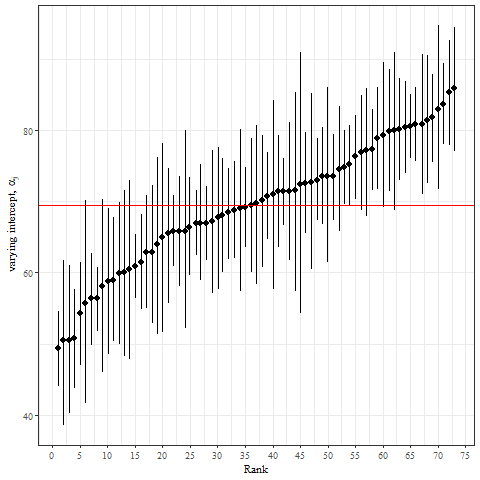
\includegraphics[width=10cm,height=10cm,keepaspectratio]{./graphics/ranking.png}
	%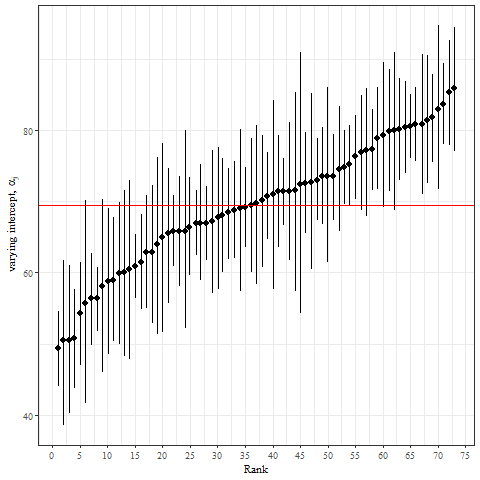
\includegraphics[width=\linewidth]{graphics/ranking.png}
	\caption{Ranking for school varying intercepts. The red line represents the mean of all the posterior means: $69.42577$.}
	\label{fig:ranking}
\end{figure}

\begin{figure}[H]
	\centering
	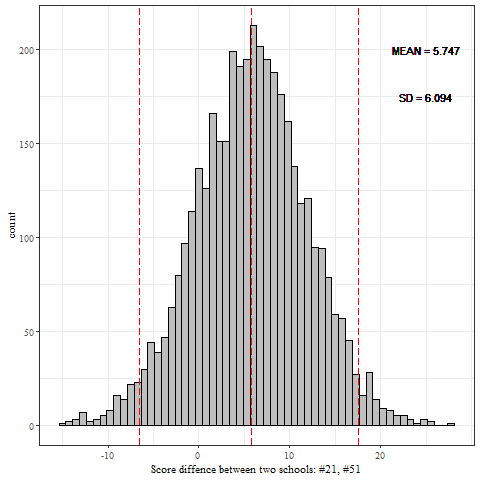
\includegraphics[width=10cm,height=10cm,keepaspectratio]{graphics/differences.png}
	\caption{}
	\label{fig:differences}
\end{figure}

\begin{figure}[H]
	\centering
	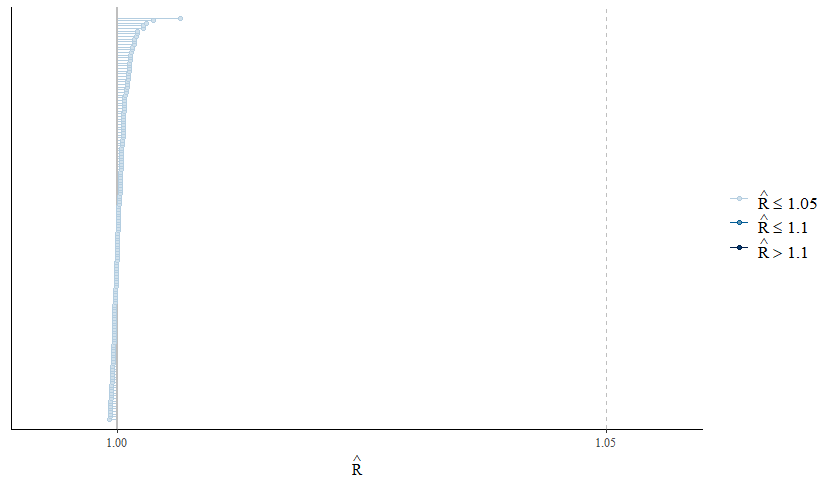
\includegraphics[width=15cm,height=15cm,keepaspectratio]{graphics/rhat.png}
	\caption{The ratio of between-chain variance to within-chain variance.}
	\label{fig:rhat}
\end{figure}


\begin{figure}[H]
  \centering
  \begin{subfigure}{0.4\linewidth}
    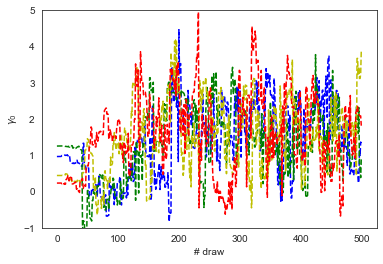
\includegraphics[width=\linewidth]{graphics/convergence_1}
    \caption{DGP 1: Draws of 4 chains}
  \end{subfigure}
  \begin{subfigure}{0.4\linewidth}
    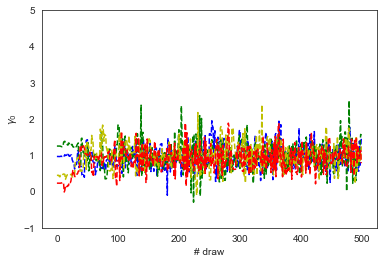
\includegraphics[width=\linewidth]{graphics/convergence}
    \caption{DGP 2: Draws of 4 chains}
  \end{subfigure}
  \caption{First 500 parameter draws of $\gamma_0$.}
  \label{fig:convergence}
\end{figure}


\begin{figure}[H]
  \centering
    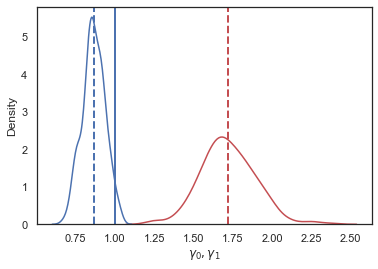
\includegraphics[width=\linewidth]{graphics/dgp_1_wrong_prior}
    \caption{Our first DGP: Impact of a wrong prior distribution on $\gamma_0$ (blue) and $\gamma_1$ (red). Graph shows densities of mean estimates;  the dotted lines are average estimates}
  \label{fig:wrong_prior_dgp1}
\end{figure}

\begin{figure}[H]
  \centering
  \begin{subfigure}[b]{0.3\linewidth}
    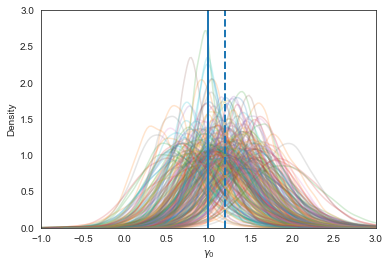
\includegraphics[width=\linewidth]{graphics/posterior_plot_gamma0_wrong}
    \caption{ N=200, J=10}
  \end{subfigure}
  \begin{subfigure}[b]{0.3\linewidth}
    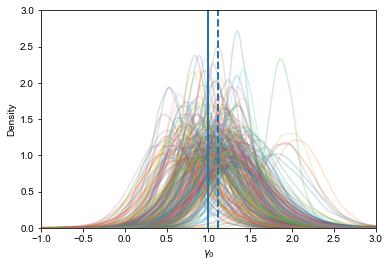
\includegraphics[width=\linewidth]{graphics/posterior_plot_gamma0_wrong_smallN}
    \caption{ N=100, J=10}
  \end{subfigure}
  \begin{subfigure}[b]{0.3\linewidth}
    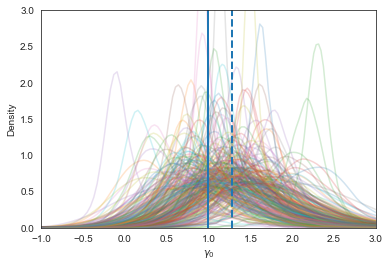
\includegraphics[width=\linewidth]{graphics/posterior_plot_gamma0_wrong_smallJ}
    \caption{N=200, J=5}
  \end{subfigure}
  \caption{Posterior densities of $\gamma_0$ with wrong prior, Blue line: True Value, Dotted line: Average Estimate}
  \label{fig:posterior_wrong_gamma0}
\end{figure}

\begin{figure}[H]
  \centering
  \begin{subfigure}[b]{0.3\linewidth}
    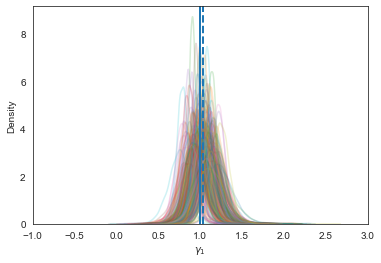
\includegraphics[width=\linewidth]{graphics/posterior_plot_gamma1_wrong}
    \caption{ N=200, J=10}
  \end{subfigure}
  \begin{subfigure}[b]{0.3\linewidth}
    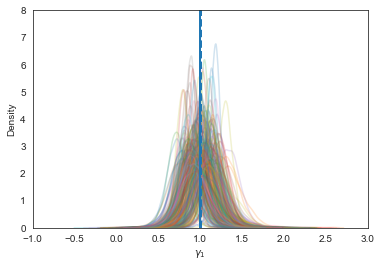
\includegraphics[width=\linewidth]{graphics/posterior_plot_gamma1_wrong_smallN}
    \caption{ N=100, J=10}
  \end{subfigure}
  \begin{subfigure}[b]{0.3\linewidth}
    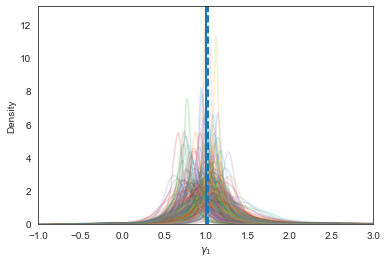
\includegraphics[width=\linewidth]{graphics/posterior_plot_gamma1_wrong_smallJ}
    \caption{N=200, J=5}
  \end{subfigure}
  \caption{Posterior densities of $\gamma_1$ with wrong prior, Blue line: True Value, Dotted line: Average Estimate}
  \label{fig:posterior_wrong_gamma1}
\end{figure}

\subsection{Tables}

\begin{table}[H]
\begin{center}
\begin{tabular}{l l}
Hamilton Monte Carlo Parameterization & DGP 1: default values\\
\hline
Number of iterations &4000  \\
Number of burn-in & 2000 \\
Number of parallell chains & 4  \\
Inital values & UNI[-2,2]  \\
target acceptance rate & 0.9  \\
max treedepth & 25 \\
\end{tabular}
\end{center}
\caption{Our default HMC parametrization for the \emph{first data generating process}. In reality we adjust values based on stan error warning, convergence tests and performance requirements.}
\label{tab:default_1}
\end{table}

\begin{table}[H]
\begin{center}
\begin{tabular}{l l}
Hamilton Monte Carlo Parameterization & DGP 2: default values\\
\hline
Number of iterations &2000  \\
Number of burn-in & 500 \\
Number of parallell chains & 4  \\
Inital values & UNI[-2,2]  \\
target acceptance rate & 0.8  \\
max treedepth & 15 \\
\end{tabular}
\end{center}
\caption{Our default HMC parametrization for the \emph{second data generating process}. In reality we adjust values based on stan error warning, convergence tests and performance requirements.}
\label{tab:default_2}
\end{table}




%BIAS analysis
\begin{table}[H]
\begin{center}
\begin{tabular}{l  l  l  l  l  l  l  }
prior & \# classes & \#  students per class & $\gamma_0$ & $\gamma_1$\\
(def. in table)  & J  & N &  [1] &  [1] \\
\hline
\hline
%$\gamma_0=1, \gamma_1=1, \mu_x=\mu_u=5,\sigma_u=\sigma_x=0.3$\\
true & 8  &  200  &  1.002  &  0.9985 \\
true & 10  &  200  &  1.0089  &  0.9835 \\
weakwrong(just 80 runs) & 10  &  200  &  0.9033  &  1.5117\\
wrong & 10  &  200  &  0.865  &  1.7222\\
uni & 15  &  200  &  1.0296  &  0.9924\\
\end{tabular}
\end{center}
\caption{DGP1:Average posterior means of the \emph{random slope model} with different class sizes and number of schools. In square brackets: True parameter values.}
\label{tab:bias_first}
\end{table}

%BIAS analysis
\begin{table}[H]
\begin{center}
\begin{tabular}{l  l  l  l  l  l  l  }
prior & \# classes & \#  students per class & $\gamma_0$ & $\gamma_1$  & $\sigma_b$ & $\sigma_y$ \\
(def. in table)  & J  & N &  [1] &  [1]  & [1] & [1] \\
\hline
\hline
%$\gamma_0=1, \gamma_1=1, \mu_x=\mu_u=0,\sigma_u=\sigma_x=3$\\
true & 10  &  200  &  1.007  &  1.0355  &  1.1424  &  1.0001\\
wrong & 10  &  200  &  1.0376  &  1.1918  &  1.1587  &  1.0001\\
weakwrong & 10  &  200  &  1.0117  &  1.0622  &  1.1579  &  1.0001\\
weakslightlywrong & 10  &  200  &  1.0084  &  1.0448  &  1.1573  &  1.0001\\
uni &10  &  200  &  1.008  &  1.0415  &  1.1609  &  1.0001\\
\hline
true &10  &  100  &  0.9907  &  0.9921  &  1.161  &  1.0008\\
wrong & 10  &  100  &  1.009  &  1.1154  &  1.1752  &  1.0008\\
weakwrong & 10  &  100  &  0.9927  &  1.0082  &  1.1767  &  1.0007\\
weakslightlywrong & 10  &  100  &  0.9905  &  0.9954  &  1.176  &  1.0007\\
uni & 10  &  100  &  0.9906  &  0.9911  &  1.1791  &  1.0008\\
\hline
true & 5  &  200  &  0.9859  &  1.014  &  1.3556  &  1.0006\\
wrong & 5  &  200  &  1.0216  &  1.2784  &  1.4418  &  1.0006\\
weakwrong & 5  &  200  &  0.9885  &  1.0768  &  1.4886  &  1.0006\\
weakslightlywrong& 5  &  200  &  0.9858  &  1.0292  &  1.4832  &  1.0006\\
uni & 5  &  200  &  0.9851  &  1.0217  &  1.5577  &  1.0006\\
\end{tabular}
\end{center}
\caption{Average  posterior means of the \emph{random slope model} with different class sizes and number of schools. In square brackets: True parameter values.}
\label{tab:bias_second}
\end{table}


% MEAN analysis
\begin{table}[H]
\begin{center}
\begin{tabular}{l l l l  l}
prior & \# classes & \#  students per class &  $\gamma_0$ & $ \gamma_1$ \\
\hline
\hline
%$\gamma_0=1, \gamma_1=1, \mu_x=\mu_u=0,\sigma_u=\sigma_x=3$
true &10  &  200  &  [0.52,1.49]  &  [0.85,1.15]]\\
wrong& 10  &  200  &  [0.69,1.64]  &  [0.89,1.18]\\
weakwrong & 10  &  200  &  [0.49,1.57]  &  [0.84,1.15]]\\
weakslightlywrong & 10  &  200  &  [0.46,1.55]  &  [0.84,1.14]\\
uni &10  &  200  &  [0.46,1.56]  &  [0.83,1.15]\\
\hline
true &10  &  100  &  [0.54,1.35]  &  [0.82,1.17]]\\
wrong & 10  &  100  &  [0.66,1.49]  &  [0.83,1.19]\\
weakwrong & 10  &  100  &  [0.49,1.42]  &  [0.81,1.18]\\
weakslightlywrong & 10  &  100  &  [0.47,1.40]  &  [0.81,1.18]\\
uni & 10  &  100  &  [0.46,1.41]  &  [0.82,1.18]\\
\hline
true & 5  &  200  &  [0.45,1.57]  &  [0.76,1.18]\\
wrong & 5  &  200  &  [0.76,1.78]  &  [0.78,1.21]\\
weakwrong &5  &  200  &  [0.33,1.74]  &  [0.75,1.19]\\
weakslightlywrong &5  &  200  &  [0.30,1.70]  &  [0.74,1.19]\\
uni & 5  &  200  &  [0.24,1.74]  &  [0.73,1.19]\\
\end{tabular}
\end{center}
\caption{[0.05,0.95] percentiles of the (mean) estimates of the \emph{random slope model} with different class sizes and number of schools. }
\label{tab:means}
\end{table}

% quantiles: add \sigma_b and \sigma_y here!!!
\begin{table}[H]
\begin{center}
\begin{tabular}{l l l l  l}
prior & \# classes & \#  students per class &  $\gamma_0$ & $ \gamma_1$ \\
\hline
\hline
true & 10  &  200  &  [0.44,1.63]  &  [0.82,1.20]\\
wrong &10  &  200  &  [0.61,1.83]  &  [0.85,1.24]\\ % 0.91
weakwrong & 10  &  200  &  [0.41,1.72]  &  [0.82,1.21] \\  %  0.9367
weakslightlywrong & 10  &  200  &  [0.39,1.70]  &  [0.81,1.20]\\ % 0.9467
uni & 10  &  200  &  [0.38,1.71]  &  [0.81,1.21]\\ % 0.9467
\hline
true &10  &  100  &  [0.43,1.56]  &  [0.75,1.23]\\
wrong&  10  &  100  &  [0.56,1.72]  &  [0.77,1.25]\\
weakwrong & 10  &  100  &  [0.39,1.63]  &  [0.75,1.24]\\
weakslightlywrong &10  &  100  &  [0.38,1.62]  &  [0.75,1.23]\\
uni & 10  &  100  &  [0.36,1.62]  &  [0.74,1.24]\\
\hline
true & 5  &  200  &  [0.19,1.84]  &  [0.64,1.34]\\
wrong &5  &  200  &  [0.47,2.24]  &  [0.67,1.42]\\
weakwrong & 5  &  200  &  [-0.02,2.24]  &  [0.58,1.40]\\
weaklightlywrong &5  &  200  &  [-0.09,2.16]  &  [0.58,1.39]\\
uni &5  &  200  &  [-0.24,2.29]  &  [0.55,1.42]\\
\end{tabular}
\end{center}
\caption{Average [0.05,0.95] percentiles of the \emph{random slope model} with different class sizes and number of schools.}
\label{tab:quantiles}
\end{table}

% coverage ratio
% MEDIAN
\begin{table}[H]
\begin{center}
\begin{tabular}{l l l l  l}
prior & \# classes & \#  students per class &  $\gamma_0$ & $ \gamma_1$ \\
\hline
\hline
true & 10  &  200  &  [0.52,1.49]  &  [0.85,1.15]\\
wrong &10  &  200  &  [0.66,1.64]  &  [0.88,1.18]\\
weakwrong & 10  &  200  &  [0.49,1.57]  &  [0.84,1.15]\\
weakslightlywrong & 10  &  200  &  [0.46,1.55]  &  [0.84,1.15]\\
uni & 10  &  200  &  [0.46,1.56]  &  [0.83,1.15]\\
\hline
true & 10  &  100  &  [0.53,1.36]  &  [0.81,1.17]\\
wrong &10  &  100  &  [0.64,1.48]  &  [0.82,1.18]\\
weakwrong & 10  &  100  &  [0.49,1.42]  &  [0.81,1.18]\\
weakslightlywrong & 10  &  100  &  [0.47,1.40]  &  [0.81,1.18]\\
uni & 10  &  100  &  [0.46,1.40]  &  [0.81,1.18]\\
\hline
true & 5  &  200  &  [0.41,1.61]  &  [0.75,1.18]\\
wrong & 5  &  200  &  [0.67,1.78]  &  [0.76,1.20]\\
weakwrong & 5  &  200  &  [0.29,1.72]  &  [0.74,1.18]\\
weakslightlywrong & 5  &  200  &  [0.27,1.70]  &  [0.74,1.18]\\
uni & 5  &  200  &  [0.23,1.73]  &  [0.74,1.18]\\
\end{tabular}
\end{center}
\caption{ [0.05,0.95] percentiles of the (median) estimates of the \emph{random slope model} with different class sizes and number of schools. }
\label{tab:median}
\end{table}

% coverage ratio
\begin{table}[H]
\begin{center}
\begin{tabular}{l l l l  l}
prior & \# classes & \#  students per class &  $\gamma_0$ & $ \gamma_1$ \\
\hline
\hline
%$\gamma_0=1, \gamma_1=1, \mu_x=\mu_u=0,\sigma_u=\sigma_x=3$
true & 10  &  200  &  0.9867  &  0.97\\
wrong & 10  &  200  &  0.97  &  0.98\\
weakwrong & 10  &  200  &  0.9767  &  0.9767\\
weakslightlywrong & 10  &  200  &  0.9833  &  0.9733\\
uni & 10  &  200  &  0.9833  &  0.9733\\
\hline
true &10  &  100  &  0.9767  &  0.9733\\
wrong & 10  &  100  &  0.9767  &  0.98\\
weakwrong & 10  &  100  &  0.97  &  0.9733 \\
weakslightlywrong &10  &  100  &  0.97  &  0.97\\
uni &10  &  100  &  0.9733  &  0.9767\\
\hline
true & 5  &  200  &  0.9833  &  0.9833\\
wrong & 5  &  200  &  0.9633  &  0.9833\\
weakwrong & 5  &  200  &  0.98  &  0.99\\
weakslightlywrong &5  &  200  &  0.9767  &  0.99\\
uni &5  &  200  &  0.98  &  0.9833\\
\end{tabular}
\end{center}
\caption{Coverage of the [0.05,0.95] percentile of the \emph{random slope model} with different class sizes and number of schools. }
\label{tab:coverage}
\end{table}


\subsection{Proofs}

\begin{proof}[Derivation of Results in Table \ref{tab:comp_uniform_bay_ml}.]
  For the normal data problem at hand the derivation of the maximum likelihood estimators, $\bar{y}$ for $\mu$ and $(n-1) s^2 / n$ for $\sigma^2$, is well known.
  We note that the "ML Variance" denotes the theoretical variance of the estimators.
  Further, the moments of the scaled inverse $\chi^2$ distributions are available in closed form.
  In particular, if $X \sim \scaledInvChi{\nu, \tau^2}$, then $\Exp{X} = \nu \tau^2 / (\nu - 2)$ and $\var{X} = 2 \nu^2 \tau^4 / ((\nu - 2)^2 (\nu - 4))$.

  Let us first consider the parameter $\mu$.
  As the t-distribution is parameterized over its mean and variance we can simply read off these values.
  Further, as the t-distribution is symmetric the MAP is equal to its mean.

  Let us now consider the parameter $\sigma^2$.
  Plugging in the respective parameters, we get
  \begin{align*}
    \Exp{\sigma^2 \mid y} = \frac{n - 1}{n - 3} \sigma^2
  \end{align*}
  directly, and
  \begin{align*}
    \var{\sigma^2 \mid y} = \frac{2 (n-1)^2}{(n-3)^2(n-5)} \sigma^4 \,.
  \end{align*}
  To get the MAP for $\sigma^2$ we need to maximize the posterior of $\sigma^2$.
  Note that we can drop any integration constants, i.e. we need to solve
  \begin{align*}
    \maximize_{x > 0} \left\{x^{-(1 + \frac{n-1}{2})} \EXP{\frac{-(n-1) s^2}{2 x}}\right\} \,,
  \end{align*}
  where the term in curly brackets is just the posterior density of $\sigma^2$ evaluated at $x$.
  Using that the constant of integration is positive we can readily see that the posterior is concave.
  Hence, differentiating with respect to $x$ and setting this to zero yields the desired result.
\end{proof}

\begin{proof}[Derivation of Results in Table \ref{tab:comp_conjugate_bay_ml}.]
  The proof from above applies here by mutatis mutandis.
\end{proof}

\begin{remark}
The subsequent proofs presented here follow \citet{gelmanbda04}; however, we contribute detailed remarks.
\end{remark}

\begin{proof}[Proof of Proposition \ref{prop:posterior_uniform}.]
  Consider first the object $\mu \mid \sigma^2, y$.
  We get
  \begin{align*}
    p(\mu \mid \sigma^2, y) \propto p(y \mid \mu, \sigma^2) p(\mu \mid \sigma^2) \propto p(y \mid \mu, \sigma^2) \,,
  \end{align*}
  where the last step follows as the priors are assumed to be independent.
  Note then
  \begin{align*}
    p(\mu \mid \sigma^2, y) &\propto \EXP{-\frac{1}{\sigma^2}\sum_i (y_i - \mu)^2} = \EXP{-\frac{n}{\sigma^2} \frac{1}{n}\sum_i (y_i^2 - 2y_i \mu + \mu^2)}\\
    &=\EXP{-\frac{n}{\sigma^2} (\bar{y^2} - 2 \bar{y} \mu + \mu^2)} \propto
    \EXP{-\frac{1}{\sigma^2 / n} (\mu - \bar{y})^2} \,,
  \end{align*}
  where $\bar{y^2} = \frac{1}{n}\sum_i y_i^2$ and the last step is only proportional as we switch $\bar{y^2}$ for $\bar{y}^2$.
  Note that proportionality here is with respect to $\mu$.
  We thus get $\mu \mid \sigma^2, y \sim \normal{\bar{y}, \sigma^2/n}$ as our first intermediate result.

  Consider now $\sigma \mid y$.
  As we already derived the joint posterior we can compute the marginal posterior of $\sigma^2$ by integrating out $\mu$.
  Note that $\sum_i (y_i - \mu)^2 = [(n-1)s^2 + n(\bar{y} - \mu)^2]$, where $s^2$ denotes the (unbiased) sample variance. Hence
  \begin{align*}
    p(\sigma^2 \mid y) &\propto \int p(\mu, \sigma^2 \mid y) \mathrm{d} \mu\\
    &\propto \int \sigma^{-(n+2)} \EXP{-\frac{1}{2\sigma^2}\sum_i (y_i - \mu)^2} \mathrm{d} \mu\\
    &= \sigma^{-(n+2)} \int \EXP{-\frac{1}{2\sigma^2}\sum_i (y_i - \mu)^2} \mathrm{d} \mu\\
    &= \sigma^{-(n+2)} \int \EXP{-\frac{1}{2\sigma^2}[(n-1) s^2 + n(\bar{y} - \mu)^2]} \mathrm{d} \mu\\
    &= \sigma^{-(n+2)} \EXP{-\frac{1}{2\sigma^2}[(n-1) s^2]} \int \EXP{\frac{1}{2\sigma^2/n}(\mu - \bar{y})^2} \mathrm{d} \mu\\
    &= \sigma^{-(n+2)} \EXP{-\frac{1}{2\sigma^2}[(n-1) s^2]} \sqrt{2 \pi \sigma^2 / n} \\
    &\propto (\sigma^2)^{-(n+1)/2} \EXP{-\frac{1}{2\sigma^2}[(n-1) s^2]} \,,
  \end{align*}
  where the second to last step follows simply by considering the constant of integration of the normal distribution of $\mu \mid \sigma^2, y$.
  Note that here we consider proportionality with respect to $\sigma^2$.
  By inspection we see that $\sigma^2 \mid y \sim \text{scaled-Inv-} \chi^2(n-1, s^2)$, which proves our first claim.

  To finish the proof we integrate the joint posterior over $\sigma^2$ to get the marginal posterior of $\mu$.
  We evaluate the integral by substitution using
  $z = \sfrac{a}{2 \sigma^2}$ with $a = (n-1)s^2 + n(\mu - \bar{y})^2$.

  Then,
  \begin{align*}
    p(\mu \mid y) &= \int_{(0, \infty)} p(\mu, \sigma^2 \mid y) \mathrm{d}\sigma^2\\
    &\propto  \int_{(0, \infty)} (\sigma^2)^{-(n+2)/2} \EXP{-\frac{1}{2\sigma^2}[(n-1) s^2 + n(\mu - \bar{y})^2]} \mathrm{d} \sigma^2\\
    &\propto \int_{(0, \infty)} (\sigma^2)^{-(n+2)/2}\EXP{-z} [(\sigma^2)^2 / a] \mathrm{d}z\\
    &= \int_{(0, \infty)} (\sigma^2)^{-(n-2)/2} / a \EXP{-z} \mathrm{d}z\\
    &= a^{-n/2}\int_{(0, \infty)} z^{(n-2)/2}\EXP{-z} \mathrm{d}z\\
    &= a^{-n/2} \, \Gamma(n/2)\\
    &\propto a^{-n/2}\\
    &= [(n-1)s^2 + n(\mu - \bar{y})^2]^{-n/2}\\
    &\propto \left[1 + \frac{1}{n-1} \frac{(\mu - \bar{y})^2}{s^2 / n}\right]^{-n/2} \,
  \end{align*}
  where $\Gamma$ denotes the gamma function (which is finite on the positive real numbers).
  This concludes the proof by implying that $\mu \mid y \sim t_{n-1}(\bar{y}, s^2/n)$,
\end{proof}


\begin{proof}[Proof of Proposition \ref{prop:posterior_conjugate}.]
Let us first state equation \ref{eq:conjugate_posterior} and the premise again.
We have to show that
\begin{align*}
  p(\mu, \sigma^2 \mid y) \propto& (\sigma^2)^{-\frac{3 + \nu_0 + n}{2}} \times\\
  & \times \EXP{-\frac{1}{2 \sigma^2} \left[\nu_0\sigma_0^2 + \kappa_0(\mu - \mu_0)^2 + (n-1)s^2 + n(\bar{y} - \mu)^2 \right]}
\end{align*}
is $\NormalscaledInvChi{\mu_n, \sigma_n^2/\kappa_n; \nu_n, \sigma_n^2}$ with $\nu_n = \nu_0 + n$, $\kappa_n = \kappa_0 + n$, $\mu_n =\frac{\kappa_0}{\kappa_0 + n}\mu_0 + \frac{n}{\kappa_0 + n}\bar{y}$, $\sigma_n^2 = \left[\nu_0 \sigma_0^2 + (n-1)s^2 + \frac{\kappa_0 n}{\kappa_0 + n} (\bar{y} - \mu_0)^2\right] /\nu_n$.
By definition of the normal-scaled-inverse-$\chi^2$ distribution $\nu_n = \nu_0 + n$ follows trivially.
Let us therefore consider the term in square brackets in the exponential.
We have to show that
\begin{align*}
  \left[\nu_0\sigma_0^2 + \kappa_0(\mu - \mu_0)^2 + (n-1)s^2 + n(\bar{y} - \mu)^2 \right] = \nu_n \sigma_n^2 + \kappa_n (\mu - \mu_n)^2 \,.
\end{align*}
Plugging in for $\sigma_n^2$ we get for the right-hand side
\begin{align*}
  \nu_n \sigma_n^2 + \kappa_n (\mu - \mu_n)^2 = \nu_0 \sigma_0^2 + (n-1)s^2 + \frac{\kappa_0 n}{\kappa_0 + n} (\bar{y} - \mu_0)^2 + \kappa_n (\mu- \mu_n)^2 \,.
\end{align*}
Therefore we only need to check
\begin{align*}
  \kappa_0(\mu - \mu_0)^2 + n(\bar{y} - \mu)^2 = \frac{\kappa_0 n}{\kappa_0 + n} (\bar{y} - \mu_0)^2 + \kappa_n (\mu- \mu_n)^2 \,.
\end{align*}
Expanding the right-hand side we get
\begin{align*}
\frac{\kappa_0 n}{\kappa_0 + n} &(\bar{y} - \mu_0)^2 + \kappa_n (\mu- \mu_n)^2\\
&=\frac{\kappa_0 n}{\kappa_n}\left[\bar{y}^2 - 2\bar{y}\mu_0 + \mu_0^2 \right] + \kappa_n \left[\mu^2 - 2\mu\mu_n + \mu_n^2 \right]\\
&=\frac{\kappa_0 n}{\kappa_n}\left[\bar{y}^2 - 2\bar{y}\mu_0 + \mu_0^2 \right] + \kappa_n \left[\mu^2 - 2\mu\frac{\kappa_0}{\kappa_n}\mu_0 - 2\mu\frac{n}{\kappa_n}\bar{y} + \frac{\kappa_0^2}{\kappa_n^2}\mu_0^2 + \frac{n^2}{\kappa_n^2} \bar{y}^2 + 2\frac{\kappa_0}{\kappa_n} \frac{n}{\kappa_n}\mu_0\bar{y} \right]\\
&=\frac{\kappa_0 n}{\kappa_n}\left[\bar{y}^2 - 2\bar{y}\mu_0 + \mu_0^2 \right] + \kappa_n \mu^2 - 2\mu \kappa_0 \mu_0 - 2\mu n\bar{y} + \frac{\kappa_0^2}{\kappa_n}\mu_0^2 + \frac{n^2}{\kappa_n} \bar{y}^2 + 2 \kappa_0 n \mu_0 \bar{y} / \kappa_n\\
&= \left(\kappa_0 \mu^2 -2\mu \kappa_0 \mu_0 \right) + \left(n \mu^2 - 2 n \mu \bar{y} \right) + \frac{\kappa_0 n}{\kappa_n}\bar{y}^2 + \frac{\kappa_0 n}{\kappa_n}\mu_0^2 + \frac{\kappa_0^2}{\kappa_n} \mu_0^2 + \frac{n^2}{\kappa_n} \bar{y}^2\\
&= \left(\kappa_0 \mu^2 -2\mu \kappa_0 \mu_0 \right) + \left(n \mu^2 - 2 n \mu \bar{y} \right) + \bar{y}^2 \left(\frac{\kappa_0 n}{\kappa_n} + \frac{n^2}{\kappa_n}\right) + \mu_0^2\left(\frac{\kappa_0 n}{\kappa_n} + \frac{\kappa_0^2}{\kappa_n}\right)\\
&= \left(\kappa_0 \mu^2 -2\mu \kappa_0 \mu_0 + \kappa_0 \mu_0^2 \right) + \left(n \mu^2 - 2 n \mu \bar{y} + n \bar{y}^2\right)\\
&=\kappa_0(\mu - \mu_0)^2 + n(\bar{y} - \mu)^2 \,,
\end{align*}
which was what we wanted.
\end{proof}

\begin{proof}[Proof of Proposition \ref{prop:marginal_posterior}.]
We continue to use the notation of the previous proof.
As in the proof of proposition \ref{prop:posterior_uniform} we first compute the distribution of $\mu \mid \sigma^2, y$ and then derive the posterior of $\sigma^2$ by integrating $\mu$ out.
Note that we actually defined $\mu \mid \sigma^2 \sim \normal{\mu_0, \sigma^2/\kappa_0}$.
Hence,
\begin{align*}
  p(\mu \mid \sigma^2, y) &\propto p(y \mid \mu, \sigma^2) p(\mu \mid \sigma^2)\\
  &\propto \EXP{-\frac{1}{2\sigma^2/n} (\mu - \bar{y})^2} \EXP{-\frac{1}{2\sigma^2/\kappa_0}(\mu - \mu_0)^2}\\
  &= \EXP{-\frac{1}{2\sigma^2}\left[n(\mu - \bar{y})^2 + \kappa_0(\mu - \mu_0)^2 \right]}\\
  &= \EXP{-\frac{1}{2\sigma^2}\left[\mu^2(\kappa_0 + n) - 2\mu(\kappa_0\mu_0 + n\bar{y}) + (\mydots) \right]}\\
  &= \EXP{-\frac{1}{2\sigma^2 / \kappa_n}\left[\mu^2 - 2\mu(\kappa_0\mu_0 + n\bar{y})/\kappa_n + (\mydots)/\kappa_n \right]}\\
  &= \EXP{-\frac{1}{2\sigma^2 / \kappa_n}\left(\mu - \mu_n^2\right) + (\mydots)}\\
  &\propto \EXP{-\frac{1}{2\sigma^2 / \kappa_n}\left(\mu - \mu_n^2\right)} \,,
\end{align*}
which implies that $\mu \mid \sigma^2, y \sim \normal{\mu_n, \sigma^2 / \kappa_n}$, where we used $(\mydots)$ to denote constants independent of $\mu$.

Now we can use this result as
\begin{align*}
  p(\sigma^2 \mid y) &= \int p(y, \sigma^2 \mid y) \mathrm{d}\mu\\
  &\propto \int (\sigma^2)^{-\frac{3 + \nu_n}{2}} \EXP{\frac{1}{2\sigma^2} \left[\nu_n \sigma_n^2 + \kappa_n(\mu_n - \mu)^2 \right]}\mathrm{d}\mu\\
  &\propto (\sigma^2)^{-\frac{3 + \nu_n}{2}} \int \EXP{\frac{1}{2\sigma^2} \nu_n \sigma_n^2}\EXP{\frac{1}{2\sigma^2 / \kappa_n} (\mu_n - \mu)^2 }\mathrm{d}\mu\\
  &\propto (\sigma^2)^{-\frac{3 + \nu_n}{2}}\EXP{\frac{1}{2\sigma^2} \nu_n \sigma_n^2} \int \EXP{\frac{1}{2\sigma^2 / \kappa_n} (\mu_n - \mu)^2 }\mathrm{d}\mu\\
  &\propto (\sigma^2)^{-\frac{3 + \nu_n}{2}}\EXP{\frac{1}{2\sigma^2} \nu_n \sigma_n^2} \sqrt{2 \pi \sigma^2 / \kappa_n}\\
  &\propto (\sigma^2)^{-(1 + \frac{\nu_n}{2})} \EXP{-\frac{1}{2\sigma^2}\nu_n\sigma_n^2}\,,
\end{align*}
from which we can conclude that $\sigma^2 \mid y \sim \scaledInvChi{\nu_n, \sigma_n^2}$.

We end the proof by deriving the marginal posterior of $\mu$ using an analogous approach as in the proof of Proposition \ref{prop:posterior_uniform}.
Define $a := \left[\nu_n\sigma_n^2 + \kappa_n(\mu_n - \mu)^2 \right]$. We solve for the posterior by integrating $\sigma^2$ out using the substitution $z = \frac{a}{2\sigma^2}$. Then
\begin{align*}
  p(\mu \mid y) &= \int_{(0, \infty)} p(\mu, \sigma^2 \mid y) \mathrm{d}\sigma^2\\
  &\propto \int_{(0, \infty)}(\sigma^2)^{-\frac{3 + \nu_n}{2}} \EXP{\frac{1}{2\sigma^2} \left[\nu_n \sigma_n^2 + \kappa_n(\mu_n - \mu)^2 \right]}\mathrm{d}\sigma^2\\
  &\propto \int_{(0, \infty)}(\sigma^2)^{-\frac{3 + \nu_n}{2}} \EXP{\frac{a}{2\sigma^2}}\mathrm{d}\sigma^2\\
  &\propto \int_{(0, \infty)}(a / 2z)^{-\frac{3 + \nu_n}{2}} \EXP{-z} \frac{a}{2 z^2} \mathrm{d}z\\
  &\propto \int_{(0, \infty)}a^{-\frac{3 + \nu_n}{2}}a z^{\frac{3 + \nu_n}{2}}z^{-2} \EXP{-z} \mathrm{d}z\\
  &= a^{-\frac{1 + \nu_n}{2}} \int_{(0, \infty)} z^{\frac{\nu_n - 1}{2}} \EXP{-z} \mathrm{d}z\\
  &= a^{-\frac{1 + \nu_n}{2}} \Gamma\left(\frac{\nu_n + 1}{2}\right)\\
  &\propto a^{-\frac{1 + \nu_n}{2}}\\
  &= \left[\nu_n \sigma_n^2 + \kappa_n(\mu_n - \mu)^2 \right]^{-\frac{1 + \nu_n}{2}}\\
  &= \left[\nu_n \sigma_n^2\left(1 + \frac{1}{\nu_n}\frac{(\mu_n - \mu)^2}{\sigma_n^2 / \kappa_n}\right) \right]^{-\frac{1 + \nu_n}{2}}\\
  &\propto \left[1 + \frac{1}{\nu_n}\frac{(\mu_n - \mu)^2}{\sigma_n^2 / \kappa_n} \right]^{-\frac{1 + \nu_n}{2}} \,,
\end{align*}
which concludes the proof by implying that $\mu \mid y \sim t_{\nu_n}(\mu_n, \sigma_n^2 / \kappa_n)$.
\end{proof}
